\section{\large Ejercicio 5: La ecuación normal del plano.}

Resuelva el siguiente problema relacionado con planos en el espacio utilizando los conceptos teóricos correspondientes y grafique la solución utilizando la herramienta GeoGebra.

Determine la ecuación normal del plano que contiene los puntos $P(4,2,7),Q(8,5,-6)$ y $R(-7,7,9)$.

\[\vec{P_0P}\cdot\vec{n}\]
\begin{itemize}
    \item Calcular el vector normal $\vec{n}$.
    \[\vec{PQ}=(8,5,-6)-(4,2,7)=(4,3,-13)\]
    \[\vec{PR}=(-7,7,9)-(4,2,7)=(-11,5,2)\]
    \[
        \vec{PQ}\times\vec{PR} = 
        \begin{vmatrix}
            i & j & k \\
            4 & 3 & -13 \\
            -11 & 5 & 2 \\
        \end{vmatrix}
    \]
    \[=(6-(-65))i-(8-143)j+(20-(-33)k)\]
    \[=71i+135j+53k\]
    \[\vec{n}=(71,135,53)\]
    \item Calculamos \(\vec{P_0P}\)
    \[
        \begin{aligned}
            P_0=(4,2,7) \\
            P=(x,y,z)  
        \end{aligned}
    \]
    \[
        \vec{P_0P}=(x-4,y-2,z-7)
    \]
    \item Multiplicar $\vec{P_0P}$ por el vector $\vec{n}$.
    \[(x-4,y-2,z-7)\cdot(71,135,53)\]
    \[71(x-4)+135(y-2)+53(z-7)=0\]
    \[71x-284+135y-270+53z-371\]
    \[71x+135y+53z-925=0\]
\end{itemize}
\begin{center}
    \textbf{solución:} $71x+135y+53z-925=0$
\end{center}

\newpage
\textbf{Grafica de la solución en GeoGebra}
\begin{figure}[ht!]
    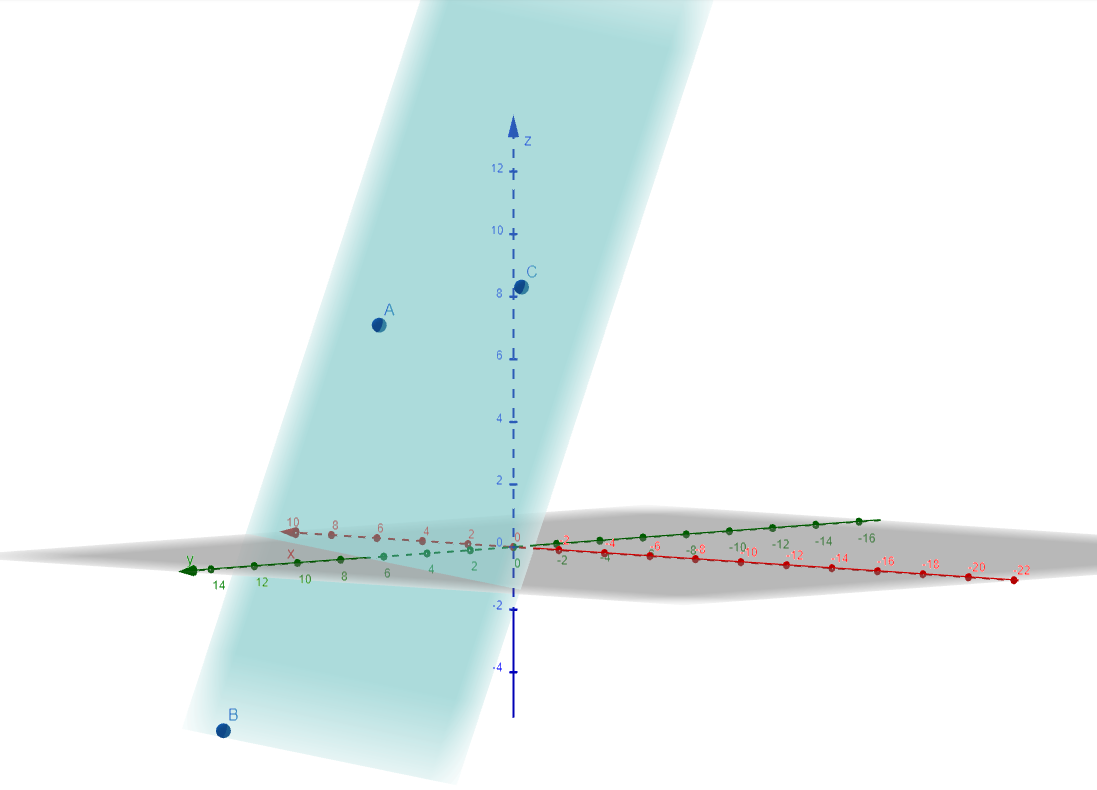
\includegraphics[width=\textwidth]{geogebra6.png}
\end{figure}
